\chapter{Implementacja}
\section{Zarządzanie projektem PDDL}
\subsection{Tworzenie projektu PDDL}
\subsection{Tworzenie nowych plików PDDL}


\section{Przetwarzanie kodu PDDL}
W specyfikacji wymagań zostały zawarte punkty dotyczące wyświetlania błędów znajdujących 
się w pliku PDDL (\ref{reqErrorDetection}) oraz prezentowania listy automatycznych\
podpowiedzi wyrazów (\ref{reqAutocompletion}).
Obie te fukcje oparte są na informacjach zawartych w kodzie źródłowym i związane
z jego analizą.

Modelem informacji umiesczonych w plikach PDDL projektu jest indeks kodu. Jest to
zbiór klas reprezentujących struktury języka PDDL takie jak domeny, problemy, akcje, czy predykaty.
Przy każdej zmianie pliku z kodem źródłowym dokonywana jest jego analiza oraz
aktualizacja indeksu. Ponadto raportowane są błędy występujące w pliku.

Pomiędzy plikami PDDL występują zależności. Aby poprawnie zinterpretować zawartość z plikiem
problemu potrzeba znać zawartość pliku domeny. Powiązanie to jest znacznie prostrze od 
powiązań pomiędzy plikami zawierającymi kod popularnych imperatywnych językach programowania.
Tymniemniej analiza plików PDDL powinna odbywać się w ramach projektu.

W środowisku Eclipse przyjęty jest standardowy sposób rozwiązywania zadania przetwarzania
kodu. Polega on na definicji klasy budowniczego (ang. \emph{builder}). Klasa ta
zawiera kod, który będzie wykonywany przy każdej zmianie zasobu. Zasobem
może być plik lub folder. Budowniczowie
są przypisani do projektu i zawsze działają w jego kontekście.

Budowniczemu przekazywany jest obiekt typu \texttt{IResourceDelta}. Jest to drzewowa
struktura zawierająca zmiany dotyczące zasobów. Na jej podstawie można określić, 
które zasoby zostały dodane, zmodyfikowane lub usunięte. Budowniczy PDDL wywołuje analizator
kodu PDDL dla każdego nowego lub zmienionego pliku. Usunięcie pliku powoduje wykreślenie
odpowiednich informacji z indeksu.

Analizator kodu PDDL został zaimplementowany w klasie PDDLAnalyzer.
Jego struktura została przedstawiona na rysunku \ref{ana_structure}.
Przetwarzany plik PDDL jest poddawany najpierw analizie leksykalnej i zamieniany
na strumień symboli leksykalnych. Następnie, analizator składniowy tworzy abstrakcyjne
drzewo składniowe. Drzewo to poddawane jest analizie semantycznej przez dwa moduły.
Moduł indeksowania kodu tworzy indeks kodu.
Moduł sprawdzania poprawności semantycznej wykrywa błędy na podstawie indeksu oraz
drzewa składniowego. Podprogram obsługi błędów zbiera informacje o błędach występujących
na poszczególnych etapach analizy oraz wyświetla je użytkownikowi.

\begin{figure}[h]
  \centering
    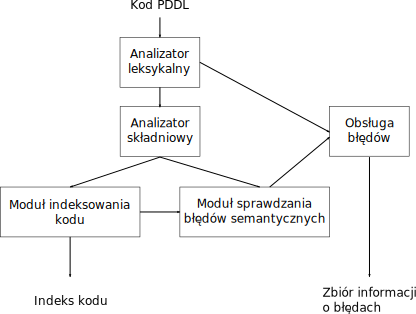
\includegraphics{img/ana_structure.pdf}
    \caption{Struktura analizatora kodu PDDL}
    \label{ana_structure}
\end{figure}

\begin{sloppypar}
Analizator przetwarza pliki w języku PDDL w wersji 1.2 \cite{pddl}. Wspieranymi wymaganiami
są \textbf{:strips}, \textbf{:typing}, \textbf{:disjunctive-preconditions}, \textbf{:equality},
\textbf{:existential-preconditions}, \textbf{:universal-preconditions}, \textbf{:quantified-preconditions},
\textbf{:conditional-effects}, \textbf{:fluents}, \textbf{:adl}.
\end{sloppypar}

\subsection{Analizator leksykaly i składniowy}
Analizator leksykalny i składniowy są automatycznie generowane przez narzędzie ANTLR
na podstawie gramatyki. 

Wykorzystanie generatora analizatorów ma wiele zalet. Nakład pracy poniesiony na
opracowanie gramatyki jest znacznie mniejszy niż przy ręcznej implementacji analizora.
W związku z tym zmniejsza się ryzyko popełnienia błędu. Ponadto, wygenerowane analizatory są 
wydajne. Gramatykę można także przeanalizować pod kątem występowania niejednoznaczności
składniowych
oraz konstrukcji trudnych do analizy. Istotną kwestią jest także to, że
języki zmieniają się w czasie. Dodawane są nowe konstrukcje i zadania. Implementację
bazującą na gramatyce można w łatwy sposób zmienić.

Generator analizatorów ANTLR posiada szereg zalet, które zadecydowały o jego wyborze.
Największe znaczenie miała rozbudowana obsługa błędów w wygenerowanych analizatorach.
Domyślne komunikaty o błędach składniowych są czytelne dla użytkowników końcowych.
Można je też zastąpić własnymi komunikatami. Do ich generacji można wykorzystać tę samą 
informację kontekstową, która służy do utworzenia treści domyślnych komunikatów.
Oprócz tego wykorzystane zostało wbudowane w ANTLR narzędzie do implementacji
terstów jednostkowych gUnit.

Kolejną zaletą narzędzia ANTLR jest dostępność środowiska ANTLRWorks, w którym
rozwijano gramatykę języka PDDL. Udostępnia 
ono edytor kolorujący składnię oraz automatycznie formatujący kod. Możliwe jest
testowe uruchamianie analizatora lub wybranej reguły dla fragmentu kodu PDDL.
Wyświetlana jest wówczas wizualizacja drzewa wyprowadzania. Jest to bardzo przydatne
podczas wyszukiwania błędów gramatyki.

Do implementacji analizatorów wykorzystano specyfikację języka PDDL w wersji 1.2 \cite{pddl}.
Dokument zawiera opis składni za pomocą notacji Backusa-Naura. Na jego podstawie opracowano
gramatykę przetwarzaną przez ANTLR.

\begin{sloppypar}
Pliki związane z analizą programu źródłowego znajdują się w pakiecie 
\texttt{pl.poznan.put.cs.gui4pdddl.parser}.
Plik \texttt{PDDL.g} zawiera połączony opis analizatora
składniowego i leksykalnego.  %Można napisać że duże litery to terminale
Na jego podstawie generowane są klasy \texttt{PDDLLexer} i \texttt{PDDLParser}.
Analizator składniowy tworzy abstrakcyjne drzewo składniowe, używając mechanizmów
wbudowanych w ANTLR.
\end{sloppypar}


Analizatory LL, generowane przez ANTLR, mają własność \emph{prefiksu żywotnego}.
Oznacza to, że błąd jest wykrywany w miejscu, w którym prefiks wejścia nie może
być prefiksem żadnego napisu w danym języku. Miejsce to znajduje się blisko miejsca
wystąpienia błędu.

Kiedy zostanie wykryty błąd, zostaje wywołana procedura obsługi. W klasach 
PDDLLexer i PDDLParser tworzony jest obiekt klasy \emph{PDDLError}. Zawiera
ona informacje o miejscu wystąpienia błędu oraz komunikat diagnostyczny. Użyto
domyślnej treści komunikatów. Obiekt dodawany jest do listy błędów. 

Analiza kodu nie powinna być przerywana przy napotkaniu pierwszego błędu. Takie
działanie byłoby uciążliwe. Dlatego też, po wystąpieniu błędu analizator podejmuje
próbę odzyskania kontroli. Analizator leksykalny przechodzi w tryb paniki. Po napotkaniu 
błędu pomija znaki na wejściu aż do napotkania znaku, który pownien wystąpić.

Domyślna strategia odzyskiwania kontroli przez analizatory składniowe wygenerowane 
za pomocą ANTLR jest opisana w \cite{antlr}. Ze względu na specyfikę języka PDDL
należało wprowadzić pewne poprawki. Pierwsza z nich dotyczy błędów zgłoszonych na końcu pliku.
Zwykle są to błędy wynikające z niedopasowania liczby nawiasów.
Metoda \texttt{recoverFromMismatchedToken} wstawia symbole \textbf{)} tak długo, jak to jest konieczne.
Druga poprawka dotyczy sytuacji, kiedy w miejscu wystąpieniu błędu nie możebyć użyta żadna
z produkcji. Metoda \texttt{recover} próbuje opuścić bieżący poziom zagnieżdżenia.

\begin{Code}
\begin{lstlisting}[language=LISP,frame=single,label=ana_code, caption=Kod PDDL zawierający błąd składniowy]
(define (problem p1)
	(:domain world-of-blocks)
	(:objects a b)
	(:init
		(clear b)
		(on-top c b)
		(on-top b a)
	)
	(:goal
		(ann
			(clear a)
			(on-top a b)
      (on-floor b)
		)
	)
)
\end{lstlisting}
\end{Code}

W kodzie z przykładu \ref{ana_code} znajduje się błąd składniowy. Zamiast słowa kluczowego \textbf{and}
wystąpił w 10 linii ciąg znaków ann. W tym miejscu zostanie zgłoszony błąd. Metoda odzyskiwania kontroli
pominie zagnieżdżone konstrukcje i spowoduje przejście do linii 14.

\subsection{Tworzenie indeksu}
\label{subsec:indeks}
Na podstawie abstrakcyjnego drzewa składniowego tworzony jest indeks kodu. 
Gramatyka opisująca analizator drzewowy znajduje się w pliku \texttt{PDDLModelBuilder.g}.

Klasy będące modelami struktur PDDL i wchodzące w skład indeksu znajdują się w pakiecie
\texttt{pl.poznan.put.cs.gui4pddl.codemodel}. Schemat zależności pomiędzy tymi klasami
przedstawiony jest na rysunku \ref{ana_model}. Wszystkie klasy zawierają metody dostępu
do pól.

\begin{figure}[h]
  \centering
    \includegraphics[width=\textwidth]{img/ana_model.pdf}
    \caption{Klasy współtworzące indeks kodu}
    \label{ana_model}
\end{figure}

Indeks kodu przyporządkowany jest projektowi. Znajdują się w nim informacje strukturalne dotyczące każdego
z plików PDDL w projekcie. Istnieją dwa interfejsy związane z indeksem. \texttt{IPDDLCodeModel}
zawiera metody służące do zadawania zapytań i wyszukiwania informacji. W \texttt{IPDDLProjectIndex}
znajdują się metody umożliwiające tworzenie i modyfikacje indeksu.

Klasa \texttt{PDDLCodeModel} implementuje oba interfejsy. Jest ona kolekcją obiektów klasy
\texttt{PDDLFile} reprezentujących pliki PDDL. Każdy z plików może zawierać dowolną liczbę
definicji domen, problemów lub sytuacji początkowych. 

Klasy reprezentujące definicje przechowują część informacji zawartych w pliku. Niektóre
składowe definicji zostały pominięte ze względu na fakt, że są one istotne jedynie 
dla oprogramowania wyznaczającego plan.

Klasa \texttt{PDDLType} reprezentuje typ w języku PDDL. Wspierane są typy proste, typy 
zmienne w czasie \emph{fluent}, oraz typy złożone \emph{either}.
Typ \texttt{PDDLTypedList} odpowiada liście z określeniami typów opisanej w specyfikacji PDDL.
\texttt{PDDLTypedList} stanowi listę wielkości charakterystwanych przez nazwę, będącą 
łańcuchem znaków, oraz typ.

\subsection{Wykrywanie błędów semantycznych}
Do wykrywania błędów semantycznych służy analizator drzewowy, którego gramatyka znajduje się
w pliku \texttt{PDDLSyntaxChecker.g}. Przy przechodzeniu przez abstrakcyjne drzewo składniowe
wykonywane są pewne testy mające na celu sprawdzenie, czy definicje są zgodne z opisem języka.
Wykrywane są następujące błędy semantyczne:
\begin{itemize}
\item nieznana nazwa wymagania.
\item odwołanie do nieistniejącej domeny.
\item odwołanie do nieistniejącego obiektu.
\item odwołanie do nieistniejącego typu.
\item odwołanie do obiektu niezgodne z jego typem.
\item odwołanie do nieistniejącego predykatu.
\item odwołanie do nieistniejącej zmienej.
\item niewykorzystanie zmiennej użytej w definicji akcji.
\end{itemize}

Na pliki w projekcie PDDL nałożone jest dodatkowe ograniczenie. Nazwa pliku zawierającego 
domenę powinna odpowiadać nazwie domeny lub być równa \texttt{domain.pddl}. Dzięki temu 
możliwe jest jednoznaczne znalezienie powiązania pomiędzy domenami a problemami. W przypadku
niespełnienia tego ograniczenia, generowane jest ostrzeżenie.

\subsection{Obsługa błędów}
W programie Eclipse można oznaczać położenie w plikach za pomocą znaczników (ang. \emph{marker}). W ten sposób
środowiska programistyczne dla Javy i C++ wyświetlają informacje o błędach.

Znaczniki są widoczne na lewym marginesie edytora oraz w widoku problemów. Dodanie znaczników
nie modyfikuje plików, ponieważ są one przechowywane jako metadane projektu. Podczas edycji,
znaczniki są uaktualniane. Oznacza to, że mogą zostać usunięte lub przemieszczone wraz z linią
kodu, której dotyczą.

Narzędzie GUI4PDDL również używa znaczników do prezentacji informacji o błędach. Po zakończeniu 
analizy, przeglądane są listy błędów przechowywane w analizatorach. Na ich podstawie tworzone
są znaczniki. Sposób wyświetlania informacji o błędach przedstawiony jest na rysunku \ref{ana_markers}.

\begin{figure}[h]
  \centering
    \includegraphics[scale=0.5]{img/ana_markers.png}
    \caption{Wyświetlanie błędów w kodzie PDDL}
    \label{ana_markers}
\end{figure}


\subsection{Wyznaczanie listy automatycznych podpowiedzi}
\begin{sloppypar}
Podczas pracy z plikiem PDDL, edytor wyświetla listę podpowiedzi. Klasy związane z wyznaczaniem
pozycji na tej liście zawarte są w pakiecie \texttt{pl.poznan.put.cs.gui4pddl.codecompletion}.
\end{sloppypar}

Do wyznaczenia listy podpowiedzi potrzebne są dwie informacje. Jedną z nich jest indeks kodu.
Drugą stanowi kontekst, określający miejsce w edytowanym kodzie źródłowym. Algorytm obliczający 
listę podpowiedzi ustala na podstawie kontekstu, który symbol leksykalny powinien wystąpić w miejscu 
wywołania. Następnie odpowiednie wyrazy wyszukiwane są w indeksie kodu. Kolekcja znalezionych 
wyrazów jest porządkowana alfabetycznie i przekazywana edytorowi.

W narzędziu GUI4PDDL kontekst zaimplementowany został jako klasa \texttt{PDDLCodeCompletionContext}.
Przechowuje on rodzaj definicji (problem, domena,
sytuacja początkowa), nazwę definiowanego obiektu oraz stos list wyrazów. Każdy poziom stosu odpowiada
poziomowi zagnieżdżenia konstrukcji języka. Listy składają się z wyrazów występujących na danym poziomie
zagnieżdżenia przed miejscem bieżącym.

\begin{Code}
\begin{lstlisting}[language=LISP,frame=single,label=ana_completions, caption=Edytowany kod PDDL]
(define (problem rubik-01)
   (:domain rubik-1d)
   (:objects v1 v2 v3 v4 v5 v6)
   (:init
        (pos1 v1)
        (pos2 
\end{lstlisting}
\end{Code}

\begin{figure}[h]
  \centering
    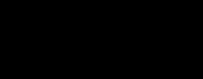
\includegraphics{img/ana_completion.pdf}
    \caption{Kontekst dla ostatniej pozycji z listingu \ref{ana_completions}}
    \label{ana_context}
\end{figure}

Rozważmy następującą sytuację. Wyznaczanie listy podpowiedzi zostało wywołane w kodzie przedstawionym
na listingu \ref{ana_completions} na końcu pliku. Dane zawarte w wyznaczonym kontekście zamieszczone
są na rysunku \ref{ana_context}. Z kontestu wynika, że edytowana jest definicja domeny o nazwie
\texttt{rubik-01}. Kursor znajduje się w strukturze będącej na trzecim poziomie zagnieżdżenia.
 Na tym poziomie,
przed kursorem znajduje się jeden wyraz \texttt{pos2}. Znajdujące się na stosie znaki \texttt{(} 
reprezentują zagnieżdżone struktury, które nie są strukturami nadrzędnymi dla bieżącej konstrukcji.

Algorytm wyznaczania listy podpowiedzi został zaimplementowany w klasie \texttt{PDDLCodeCompletionManager}.
Zawarta jest w niej kolekcja dostawców podpowiedzi. Dostawcy, implementujący interfejs
\texttt{IPDDLCodeCompletionProvider} uzupełniają listę podpowiedzi na podstawie kontekstu 
o pozycje związane z pojedynczym rodzajem symboli leksykalnych. Wyznaczanie listy podpowiedzi polega 
więc na obliczeniu kontekstu i przekazaniu go wszystkim dostawcom.

W narzędziu GUI4PDDL zaimplementowane zostało podpowiadanie:
\begin{itemize}
\item obiektów
\item predykatów
\item słów kluczowych
\item typów
\item wymagań
\item zmiennych
\end{itemize}

\section{Edytor}
Edytor kodu we wtyczce GUI4PDDL zajmuje się kolorowaniem kodu, dopasowywaniem nawiasów oraz podpowiedziami kodu. Automatyczne wcięcia zaimplementowane są domyślnie w edytorze Eclipse, tak więc po wpisaniu znaku nowej linii kursor automatycznie ustawia się w takiej odległości od lewej krawędzi, jak w poprzedniej linii kodu.
\subsection{Kolorowanie kodu}
\begin{figure}[h]
  \centering
    \includegraphics{img/colored-code.png}
    \caption{Pokolorowany kod PDDL}
    \label{ana_structure}
\end{figure}
Aby zaimplementować kolorowanie kodu, wykorzystano metody ze środowiska programistycznego Eclipse. Dokument wstępnie dzielony jest na partycje, czyli fragmenty kodu mające charakterystyczne cechy. Następnie każda partycja jest dzielona na tzw. tokeny. W GUI4PDDL kod podzielony jest na 2 partycje. Pierwsza partycja obejmuje komentarze. Klasa PDDLPartitionScanner znajduje fragmenty kodu rozpoczynające się od znaku ";", np.  ";testowy kometarz". Od tego znaku aż do końca linii, zgodnie z gramatyką języka PDDL, tekst traktowany jest jako komentarz.
\begin{figure}[h]
  \centering
    \includegraphics{img/comments.png}
    \caption{Komentarze są możliwe również na końcu linii}
    \label{ana_structure}
\end{figure}
Pozostałe fragmenty kodu poddawane są dalszej analizie. Klasa DefaultScanner zawiera listę słów kluczowych oraz definicje tokenów i reguł. Reguły wywoływane są w specjalnej kolejności, by wykluczyć błędne dopasowanie kodu do tokena. Pierwsza reguła szuka słów kluczowych zaczynających się znakiem ":".  Od tego znaku, aż do końca słowa (dopuszczalny myślnik) tekst przyrównywany jest do listy słów kluczowych. Jeśli słowo znajduje się na liście, fragment kodu oznaczony jest tokenem valueToken.
 W przeciwnym wypadku edytor "cofa się" na początek analizowanego kodu i klasa DefaultScanner wywołuje kolejną regułę. Następna metoda znajduje fragmenty kodu rozpoczynające się na znak "?".  Podobnie jak w przypadku pierwszej reguły, skaner odczytuje kolejne litery lub cyfry (dopuszczalne znaki specjalne to kropka oraz myślnik). Taki fragment oznaczony jest jako zmienna w języku PDDL. Tekst otrzymuje token variableToken.
\begin{figure}[h]
  \centering
    \includegraphics{img/values-color.png}
    \caption{Słowa kluczowe oznaczone tokenem valueToken}
    \label{ana_structure}
\end{figure}
\begin{figure}[h]
  \centering
    \includegraphics{img/variable-color.png}
    \caption{Słowa kluczowe oznaczone tokenem variableToken}
    \label{ana_structure}
\end{figure}
\begin{figure}[h]
  \centering
    \includegraphics{img/bracket-color.png}
    \caption{Nawiasy oznaczone tokenem bracketToken}
    \label{ana_structure}
\end{figure}
Kolejna reguła wyszukuje stałe słowa, takie jak np. define. Metoda ta działa identycznie, jak w przypadku valueRule. Fragment kodu dopasowany jest do listy słów kluczowych z listy keywords. Elementy pasujące do reguły otrzymują token keywordToken. Reguła dotycząca nawiasów to BracketRule. Ponieważ w języku PDDL nie dopuszcza się znaków "(" oraz ")" w nazwach zmiennych, ani słowach kluczowych, BracketRule analizuje znaki szukając nawiasów okrągłych. Znaki te otrzymują token bracketToken.
Przedostatnia reguła znajduje wszystkie puste znaki, wykorzystując wbudowany interfejs  IWhitespaceDetector oraz metodę klasy Character - isWhitespace(). Jeśli fragment kodu nie dostał żadnego tokenu, otrzymuje token domyślny.  Po podziale kodu na tokeny, środowisko Eclipse używając wbudowanych metod, koloruje tokeny na kolory ustalone przez użytkownika w ustawieniach, bądź domyślne, zdefiniowane w klasie Activator.
\subsection{Dopasowanie nawiasów}
\begin{figure}[h]
  \centering
    \includegraphics{img/matched-bracket.png}
    \caption{Zaznaczony nawias w parze z nawiasem spod kursora}
    \label{ana_structure}
\end{figure}
\begin{figure}[h]
  \centering
    \includegraphics{img/matched-bracket-reverse.png}
    \caption{Zaznaczanie działa w obie strony}
    \label{ana_structure}
\end{figure}
Środowisko Eclipse posiada wbudowaną metodę w klasie TextEditor, configureSourceViewerDecorationSupport. W klasie PDDLEditor zostaje ona nadpisana własną funkcją. Wykorzystano metodę setCharacterPairMatcher. Metoda ta wyszukuje rekurencyjnie kolejne pary znaków "(" oraz ")".  W edytorze dopasowane nawiasy są sparowane, więc przy zaznaczaniu jednego znaku z pary, drugi nawias otoczony jest szarą obwódką. Dzięki temu użytkownik szybko zauważy dopasowany nawias, lub jego brak.
\subsection{Podpowiadanie kodu}
Podpowiadanie składni wywoływane jest po wpisaniu dowolnej litery, znaku ":" lub po wciśnięciu kombinacji klawiszy Ctrl+Space - jest to domyślna kombinacja klawiszy w środowisku Eclipse wywołująca klasę PDDLCompletionAssistant. Klasa ta wymaga bezpośredniej współpracy z naturą wtyczki GU4PDDL. Jako domyślny asystent podpowiedzi, użyto klasy PDDLCompletionAssistant. Zawiera ona metodę computeCompletionsProposals(). Na początku metoda uzyskuje dostęp do dokumentu. Następnie obliczana jest ilość znaków, począwszy od pozycji kursora w danym momencie. Skaner tekstu przechodzi przez znaki poprzedzające kursor, aż natrafi na znak pusty, lub znak specjalny z wyłączeniem znaków ":" i "?". Wynikowy tekst jest prefixem. Następnie metoda dostaje dostęp do natury projektu. Poprzez instancję IPDDLCodeCompletionManager wywoływany jest CodeComletionManager. Ostatecznie metoda pobiera listę propozycji utworzoną przez menedżer (o czym w innym rozdziale). Lista propozycji jest filtrowana używając przygotowanego wcześniej prefixu. Lista wynikowa zawiera listę słów zaczynających się prefixem. Każda propozycja z listy wyświetlona jest w oknie kontekstowym. Użytkownik następnie wybiera jedną z nich i edytor wpisuje propozycję tuż za kursorem.




\section{Współpraca z oprogramowaniem wyznaczającym plan}
\label{sec:wspolpraca}
Zadaniem oprogramowania wyznaczającego plan (tzw. plannera) jest przetwarzanie problemów automatycznego planowania, uzyskując na wyjściu plan, czyli sekwencję akcji, umożliwiającą osiągnięcie stanu końcowego ze stanu początkowego problemu. Opis problemu wyrażony jest za pomocą języka automatycznego planowania (np. \textit{STRIPS}, \textit{PDDL}). 

W przypadku języka \textit{PDDL}, wykorzystywanego w niniejszej pracy, zadanie automatycznego planowania składa się z dwóch plików: pliku domeny, w którym opisana jest dziedzina zadania oraz pliku problemu, opisującego stan początkowy oraz docelowy. Współpraca narzędzia GUI4PDDL z plannerami wymaga więc sposobności uzyskania planu na podstawie aktualnej zawartości dwóch, wyżej wymienionych plików. Ponadto należy zagwarantować możliwość zmiany algorytmu planowania lub innych opcji, które są dostępne dla poszczególnych narzędzi. Gotowy plan powinien być również przedstawiony użytkownikowi w postaci czytelnej.

Obecnie dostępnych jest wiele plannerów, korzystających z języka \textit{PDDL}, różniących się dostępnymi algorytmami, sposobem uruchamiania, ilością oraz rodzajem przyjmowanych na wejściu argumentów, a także strukturą strumienia wyjściowego. Ze względu na to, że programy wyznaczające plan tworzone są często z przeznaczeniem na konkurs \textit{IPC} (\textit{International Planning Competition}), dotychczas nie zdefiniowano standardu uruchamiania tego typu narzędzi, który obejmowałby m.in. ujednolicenie argumentów linii poleceń, dodatkowo wykorzystywanych narzędzi, specyficznych dla systemu operacyjnego oraz formatu plików wyjściowych.

Analiza przykładowych narzędzi (\textit{FastDownward}, \textit{SATPLAN}, \textit{FastForward}) pod kątem inicjalizacji procesu planowania wykazała następujące cechy wspólne oraz różnice pomiędzy plannerami:
\begin{table}[h]
\centering
\caption{Cechy wspólne oraz różnice w uruchamianiu pomiędzy przykładowymi plannerami.}
\label{plannersTable}
\begin{tabular}{|p{6cm}|p{6cm}|}
\hline
\multicolumn{1}{|>{\centering\arraybackslash}m{6cm}|}{\textbf{Cechy wspólne}} 
    & \multicolumn{1}{>{\centering\arraybackslash}m{6cm}|}{\textbf{Różnice}} 
   \\
   \hline
\begin{itemize}
\item Narzędzia konsolowe.
\item Wymaganie wskazania ścieżek do plików domeny oraz problemu.
\item Możliwość wyboru algorytmu za pomocą argumentu wejściowego programu.
\item Tworzenie pliku wyjściowego z wynikowym planem.
\end{itemize}
&
\begin{itemize}
\item Różna liczba faz przetwarzania.
\item Różna liczba podprogramów plannera.
\item Różnice w nazewnictwie poszczególnych opcji i algorytmów.
\item Różnice w nazwie pliku wyjściowego oraz jego formatowaniu.
\end{itemize} \\
\hline
\end{tabular}
\end{table}

Biorąc pod uwagę powyższe cechy wspólne oraz wymaganie projektu, dotyczące możliwości integracji z wieloma plannerami, ze szczególnym uwzględnieniem \textit{FastDownward}, zdecydowano o stworzeniu wewnętrznego standardu uruchamiania. Standard ten opisuje postać argumentów linii poleceń dla plików plannerów, które mogą być prawidłowo powiązane z wtyczką GUI4PDDL. 

Narzędzia te wymagają podania na wejście programu ścieżek do plików domeny oraz problemu. W niektórych przypadkach konieczne jest także wskazanie nazwy algorytmu planowania. Cechy te w całości pokrywają się z wymaganiami skryptu uruchomieniowego narzędzia \textit{FastDownward}. W związku z tym, powzięto decyzję o przyjęciu formatu skryptu uruchomieniowego, analogicznego do formatu skryptu \texttt{plan}, znajdującego się w katalogu \texttt{src} \textit{FastDownward}. Skrypt (bądź bezpośrednio plik wykonywalny plannera) przeznaczony do integracji z wtyczką GUI4PDDL musi więc przyjmować następujące argumenty wejściowe w odpowiedniej kolejności:

\noindent
\centerline{\texttt{<ścieżka\_do\_domeny>}\textvisiblespace\texttt{<ścieżka\_do\_problemu>}\textvisiblespace\texttt{<argumenty\_planowania>}}


\noindent
gdzie:
\begin{itemize}
\item \textbf{\texttt{<ścieżka\_do\_domeny>}} -- ścieżka do pliku domeny danego zadania automatycznego planowania.
\item \textbf{\texttt{<ścieżka\_do\_problemu>}} -- ścieżka do pliku problemu, zdefiniowanego na dziedzinie wskazanej w podanym jako pierwszy argument pliku domeny.
\item \textbf{\texttt{<argumenty\_planowania>}} -- dowolne argumenty plannera, na przykład dotyczące wyboru algorytmu planowania.
\end{itemize}
Narzędzia uruchamiane według innego schematu nie będą prawidłowo zintegrowane z GUI4PDDL. W takim przypadku należy przygotować skrypt powłoki systemu operacyjnego, który dostosuje sposób inicjalizacji procesu planowania do przedstawionego powyżej. Dzięki zastosowaniu funkcji systemowych (roz.~\ref{subsec:przerywanie}) istnieje możliwość kontroli nad tego typu skryptami z poziomu \textit{Eclipse}, włączając uruchamiane przez nie podprocesy.

Jak wspomniano, planner \textit{FastDownward} w wersji dla systemów z rodziny \textit{Linux} posiada odpowiedni plik uruchomieniowy w katalogu \path{src} instalacji. W przypadku systemu \textit{Windows} należy stworzyć osobny program wsadowy (ang \textit{batch file}). Przykładowa forma takiego pliku znajduje się w katalogu \path{resources} projektu \texttt{pl.poznan.put.cs.gui4pddl}.

Analogiczny skrypt uruchomieniowy można wykonać również dla innego oprogramowania wyznaczającego plan, np. \textit{SATPLAN}.
  
\begin{Code}
\begin{lstlisting}[language=bash,frame=single,caption={Przykładowy skrypt uruchomieniowy (skrypt \textit{bash} dla systemu \textit{Linux}) dla plannera \textit{SATPLAN}}.]
#!/bin/bash
set -e
BASEDIR="$(dirname "$0")"

function die {
    echo "$@" 1>&2
    exit 1
}

function usage {
    die "usage: $(basename "$0") DOMAIN_FILE PROBLEM_FILE SEARCH_OPTION ..."
}

# Paths to planner components
SATPLAN="$BASEDIR/satplan"

if [[ "$#" < 2 ]]; then
    usage
fi

DOMAIN=$1
PROBLEM=$2
shift 2

echo "Running SATPLAN"
"$SATPLAN" -domain "$DOMAIN" -problem "$PROBLEM" "$@"
echo
\end{lstlisting}
\end{Code}

Poza określonym formatem argumentów linii poleceń, każdy planner musi zapewnić możliwość zapisu uzyskanego planu do pliku w postaci czytelnej, co jest wykorzystywane w przeglądarce planów, opisanej w rozdziale~\ref{subsec:uruchamianie}.

\subsection{Konfiguracja zewnętrznego oprogramowania}
\label{subsec:konfiguracja}
Istnienie zróżnicowanego oprogramowania, pozwalającego wyznaczyć plan wymaga możliwości integracji ze środowiskiem programistycznym. Platforma \textit{Eclipse} zapewnia standardową opcję uruchamiania zewnętrznych narzędzi z poziomu menu \textit{Run} aplikacji, bądź skrótów znajdujących się na pasku narzędziowym lub menu kontekstowym edytowanego pliku. W wielu wtyczkach, rozszerzających \textit{Eclipse} o obsługę języków programowania ogólnego przeznaczenia (\textit{Java}, \textit{C++}), opcja ta odpowiada za rozpoczęcie procesu kompilacji. Biorąc pod uwagę podobieństwo procesu planowania do kompilacji oraz przyzwyczajenia użytkowników, zdecydowano o wprowadzeniu w projekcie GUI4PDDL analogicznego sposobu uruchamiania plannera i jego konfiguracji.

Zanim możliwa będzie aktywacja planowania z poziomu \textit{Eclipse}, należy skonfigurować planner, wybierając z menu \textit{Window}, opcję \textit{Preferences}, a następnie w otwartym oknie, rozwijając listę \textit{PDDL} wybrać element \textit{Planners}.

\begin{figure}[h!]
    \centering
    \includegraphics[width=\textwidth]{img/planner_preferences_window}
    \caption{Widok okna konfiguracji plannera.}
    \label{fig:preferences_window}
\end{figure}
Standardowo, dostępny jest wstępnie skonfigurowany planner \textit{FastDownward}. Okno preferencji udostępnia następujące opcje:
\begin{enumerate}
\item Wybór plannera domyślnego. Włączenie tej opcji, powoduje, że przy każdym uruchomieniu procesu planowania na plikach domeny i problemu, wykorzystany będzie wskazany w tym polu planner wraz z odpowiednim algorytmem planowania.
\item Nowa konfiguracja. Przycisk ten umożliwia stworzenie nowej konfiguracji, dla innego niż bieżący plannera. Może istnieć wiele takich konfiguracji, które w trakcie uruchamiania procesu planowania można dowolnie zmieniać.
\item Nazwa konfiguracji. Pozwala na rozróżnienie poszczególnych konfiguracji. Nazwa powinna być unikalna i może składać się z liter, cyfr, spacji oraz znaków ,,.'', ,,\_'', ,,-''.
\item Ścieżka do pliku plannera. Za pomocą przycisku \textit{Browse...} należy wskazać ścieżkę do pliku wykonywalnego lub skryptu powłoki systemu operacyjnego (\textit{Linux} lub \textit{Windows}), zgodnego z formatem przedstawionym w rozdziale~\ref{sec:wspolpraca}.
\item Argumenty plannera. W pierwszej kolumnie znajduje się czytelna dla użytkownika nazwa argumentu, w szczególności nazwa wykorzystywanego algorytmu planowania, która będzie używana jako prosty odpowiednik argumentu linii poleceń, znajdującego się w drugiej kolumnie. Parametry wiersza poleceń danego plannera wpisane muszą być w sposób identyczny, jak przy wpisywaniu ich podczas uruchamiania w konsoli.
\item Nowy argument. Przycisk ten umożliwia dodanie nowego argumentu linii poleceń plannera wraz z jego nazwą.
\item Edycja argumentu. Pozwala na edycję aktualnie zaznaczonego argumentu plannera.
\item Usunięcie argumentu. Pozwala na usunięcie aktualnie zaznaczonego argumentu plannera.
\item Usunięcie konfiguracji plannera. Przycisk ten usuwa bieżącą konfigurację. Nie ma możliwości cofnięcia tej operacji, dlatego przed jej wykonaniem wyświetlone zostaje pytanie, potwierdzające chęć usunięcia konfiguracji.
\item Wzorzec pliku planu. Okno to umożliwia zdefiniowanie wyrażenia regularnego, dotyczącego nazwy pliku wynikowego planu, powstałego w rezultacie działania bieżącego plannera. Prawidłowy wzorzec pozwala na wykrycie plików planów i bezpośrednie ich wyświetlenie przy pomocy przeglądarki planów (roz.~\ref{subsec:uruchamianie}).
\begin{figure}[h!]
    \centering
    \includegraphics[width=0.8\textwidth]{img/plan_view_dialog}
    \caption{Widok okna konfiguracji przeglądarki planów.}
    \label{fig:plan_view_window}
\end{figure}
\begin{enumerate}
\item Wyrażenie regularne. Wzorzec opisujący nazwę pliku wynikowego planu. Planner \textit{FastDownward} standardowo generuje pliki planów o nazwie \texttt{sas\_plan.}, a w przypadku większej ilości planów kolejno \texttt{sas\_plan.1}, \texttt{sas\_plan.2}..., dlatego wyrażenie obejmujące te nazwy ma postać \texttt{sas\_plan.*}. Dla narzędzia \textit{SATPLAN} wzorzec ma postać \texttt{-problem\_file\_name-\textbackslash.pddl\textbackslash.soln} (opis wzorca \texttt{-problem\_file\_name-} znajduje się poniżej), ponieważ generuje pliki o nazwie \texttt{<nazwa\_pliku\_problemu>.pddl.soln}.
\item Wzorzec katalogu roboczego. Przycisk ten powoduje wstawienie w bieżącym miejscu kursora, ciągu \texttt{-working\_directory-}, który w czasie procesu planowania zamieniany jest na aktualną nazwę katalogu roboczego plannera (roz.~\ref{subsec:uruchamianie}). Opcja ta pozwala na wykrycie plików wynikowych, które jako swoją nazwę przyjmują nazwę bieżącego katalogu.
\item Wzorzec nazwy projektu. Przycisk ten powoduje wstawienie w bieżącym miejscu kursora, ciągu \texttt{-project\_name-}, który w czasie planowania zamieniany jest na nazwę projektu \textit{Eclipse}, w którym znajdują się przetwarzane pliki domeny oraz problemu.
\item Wzorzec nazwy pliku domeny. Przycisk ten powoduje wstawienie w bieżącym miejscu kursora, ciągu \texttt{-domain\_file\_name-}, który w czasie planowania zamieniany jest na nazwę pliku domeny, wykorzystywanej w tym przetwarzaniu, bez rozszerzenia \texttt{.pddl}.
\item Wzorzec nazwy pliku problemu. Przycisk ten powoduje wstawienie w bieżącym miejscu kursora, ciągu \texttt{-problem\_file\_name-}, który w czasie planowania zamieniany jest na nazwę pliku problemu, wykorzystywanego w tym przetwarzaniu, bez rozszerzenia \texttt{.pddl}.
\end{enumerate}
\end{enumerate}

Minimalna konfiguracja plannera, możliwa do zapisu składa się z prawidłowej nazwy oraz ścieżki do pliku programu. Zachowanie utworzonych lub zmodyfikowanych ustawień odbywa się po naciśnięciu przycisku ,,OK''.
Wszystkie konfiguracje zapisywane są w tzw. obszarze stanu (ang. \textit{state area}) przestrzeni roboczej (ang. \textit{workspace}) w folderze \path{planner_preferences}. 

Ścieżka do tego katalogu ma następującą postać:

\noindent
\centerline{\path{<l_p_rob>/.metadata/.plugins/pl.poznan.put.cs.gui4pddl/planner_preferences}}

\noindent
gdzie:

\noindent
\textbf{\path{<l_p_rob>}} -- lokalizacja przestrzeni roboczej.

Każda konfiguracja ustawień plannera zapisywana jest w osobnym pliku o nazwie analogicznej do wpisanej w oknie preferencji. Ze względu na łatwość modyfikacji, elastyczność w przechowywaniu listy argumentów oraz odporność na zmiany, jako format zapisu danych wybrano \textit{XML}. Do tego typu serializacji, wykorzystane zostało \textit{API} dołączone do platformy \textit{Eclipse} -- \textit{Memento}. W tej formie zapisywane są wszystkie informacje o konfiguracji, z wyjątkiem ustawień domyślnego plannera, które zachowywane są przy pomocy standardowego \textit{API} \textit{Eclipse} do zapisu preferencji -- \textit{Preferences}.

\begin{Code}
\begin{lstlisting}[language=XML,frame=single,label={lst:preferencje_plannera},caption={Przykładowa konfiguracja plannera FastDownward w postaci XML}]  % Start your code-block
<?xml version="1.0" encoding="UTF-8"?>
<PlannerPreferences 
	PlanViewFilePattern="sas_plan.*" 
	PlannerFilePath="/home/user/fast-downward/src/plan" 
	PlannerName="FastDownward">
	<PlannerArguments>
		<PlannerArgumentsEntry 
			PlannerArgumentKey="A* blind heuristic" 
			PlannerArgumentValue="--search &quot;astar(blind())&quot;"/>
		<PlannerArgumentsEntry 
			PlannerArgumentKey="ipc seq-sat-lama-2011" 
			PlannerArgumentValue="ipc seq-sat-lama-2011"/>
	</PlannerArguments>
</PlannerPreferences>
\end{lstlisting}
\end{Code}

\subsection{Uruchamianie zewnętrznego oprogramowania}
\label{subsec:uruchamianie}

Inicjalizacja oprogramowania wyznaczającego plan odbywa się poprzez wbudowany w \textit{Eclipse} mechanizm skrótów uruchamiania (ang \textit{Launch Shortcuts}). Rozszerzenie wtyczki o tego typu element pozwala na wywołanie zewnętrznych narzędzi przy pomocy menu \textit{Run} lub \textit{Debug}, a także przycisku znajdującego się na pasku narzędziowym lub menu kontekstowego edytowanego pliku.
\begin{figure}[h!]
    \centering
    \includegraphics[width=0.9\textwidth]{img/running_options_menu_toolbar}
    \caption{Możliwość uruchomienia zewnętrznego oprogramowania z poziomu menu ,,Run'' oraz przycisku na pasku narzędziowym.}
    \label{fig:running_options_menu_toolbar}
\end{figure}

\begin{figure}[h!]
    \centering
    \includegraphics[width=0.9\textwidth]{img/running_options_context_menu}
    \caption{Możliwość uruchomienia zewnętrznego oprogramowania z poziomu menu kontekstowego edytowanego pliku.}
    \label{fig:running_options_context_menu}
\end{figure}

Podczas pierwszego uruchomienia zewnętrznego programu na aktualnie edytowanych plikach, tworzona jest nowa konfiguracja uruchamiania (ang. \textit{Run Configuration}). W przypadku, gdy opcja zastosowania domyślnego plannera (konfiguracja plannera, roz. \ref{subsec:konfiguracja}) nie jest ustawiona, należy w wyświetlonym oknie (rys. \ref{fig:run_configuration_window}) uzupełnić tę konfigurację o nazwę i argument plannera, który będzie wykorzystany w procesie planowania. 

\begin{figure}[h!]
    \centering
    \includegraphics[width=0.9\textwidth]{img/run_configuration_window}
    \caption{Okno konfiguracji uruchamiania.}
    \label{fig:run_configuration_window}
\end{figure}

Jeżeli uruchomienie nastąpiło na pliku problemu (za pomocą globalnego menu \textit{Run} lub przycisku na pasku narzędziowym, gdy plik problemu był otwarty w edytorze, bądź poprzez wybranie z menu kontekstowego pliku problemu opcji \textit{Run as}, \textit{PDDL Project}) ścieżka do odpowiadającego pliku domeny w projekcie zostanie automatycznie wykryta za pomocą funkcji indeksu kodu opisanego w rozdziale \ref{subsec:indeks}. Analogicznie w przypadku uruchomienia narzędzia na pliku domeny. W sytuacjach wyjątkowych (brak odpowiadającej domeny, więcej niż jeden pasujący problem) wyświetlane są listy wyboru:
\begin{itemize}
\item W przypadku gdy do danej domeny pasuje wiele plików problemów, wyświetla się okno wyboru ze wszystkimi pasującymi problemami.
\item W przypadku gdy do danej domeny nie pasuje żaden plik problemu, wyświetli się informująca o tym wiadomość.
\item W przypadku gdy do danego pliku problemu nie pasuje żaden plik domeny, ale w projekcie istnieją inne pliki domen, wyświetli się okno wyboru z wszystkimi plikami domen w projekcie.
\item W przypadku gdy do danego pliku problemu nie pasuje żaden plik domeny, ponieważ w projekcie nie istnieje żaden plik domeny, wyświetli się informująca o tym wiadomość.
\end{itemize}

Proces planowania rozpoczyna się po wybraniu przycisku \textit{Run} w oknie konfiguracji uruchamiania (lub z pominięciem tego okna w przypadku włączenia opcji domyślnego plannera w konfiguracji plannera). Działanie plannera objawia się widocznym paskiem postępu w prawym dolnym rogu aplikacji oraz na zakładce \textit{Progress} (rys.~\ref{fig:run_progress}). Również strumień wyjściowy działającego narzędzia kierowany jest w całości do widoku \textit{Console}.

\begin{figure}[h!]
    \centering
    \includegraphics[width=0.8\textwidth]{img/run_progress}
    \caption{Pasek postępu procesu planowania.}
    \label{fig:run_progress}
\end{figure}

W razie błędów należy sprawdzić wyjście (w widoku \textit{Console}) oraz poprawność skryptu poprzez uruchomienie go w konsoli systemowej. Dobrą praktyką jest również zmiana ścieżki do przestrzeni roboczej \textit{Eclipse} w taki sposób, by nie zawierała spacji, gdyż niektóre narzędzia (np. \textit{SATPLAN}) niepoprawnie obsługują takie ścieżki.

Efektem przetwarzania jest powstanie planu, który w \textit{Eclipse} jest dostępny z poziomu przeglądarki planów (ang. \textit{Plan Browser}). Jest ona widoczna standardowo w pespektywie \textit{PDDL}, jako zakładka w dolnej części aplikacji. Każdy wiersz przeglądarki wskazuje na zakończony (powodzeniem lub niepowodzeniem) proces planowania. 

\begin{figure}[h!]
    \centering
    \includegraphics[width=0.9\textwidth]{img/plan_browser_row}
    \caption{Wiersz przeglądarki planów.}
    \label{fig:plan_browser_row}
\end{figure}

\noindent
Poszczególne kolumny oznaczają:
\begin{enumerate}
\item Nazwa projektu, który zawiera rozważany problem automatycznego planowania.
\item Nazwa domeny wykorzystywanej w rozważanym problemie automatycznego planowania. Standardowo jest to nazwa pliku domeny bez rozszerzenia \texttt{.pddl}.
\item Nazwa problemu wykorzystywanego w rozważanym problemie automatycznego planowania. Standardowo jest to nazwa pliku problemu bez rozszerzenie \texttt{.pddl}.
\item Numer ID przetwarzanego zadania o danej nazwie domeny i problemu, znajdującego się w danym projekcie. W celu możliwości zachowania poprzednich wyników planowania, każde przetwarzanie wykonywane jest w innym folderze roboczym, do którego ścieżka ma postać:

\noindent
\centerline{\path{<l_p_rob>/<project_name>/plans/<domain_name>/<problem_name>/<id>}}

\noindent
gdzie:

\begin{itemize}
\item \textbf{\path{<l_p_rob>}} -- lokalizacja przestrzeni roboczej.
\item \textbf{\path{<project_name>}} -- nazwa projektu.
\item \textbf{\path{<domain_name>}} -- nazwa domeny.
\item \textbf{\path{<problem_name>}} -- nazwa problemu.
\item \textbf{\path{<id>}} -- numer ID kolejnego przetwarzania.
\end{itemize}
Dzięki takiej strukturze katalogu roboczego użytkownik nie nadpisze omyłkowo poprzednio utworzonych wyników planowania. W przeglądarce planów powstaje zaś chronologiczna lista kolejnych uruchomień plannera, którą można swobodnie zarządzać, w tym usuwać.
\item Nazwy plików wynikowych, zawierających plan, które dopasowane są do wyrażenia regularnego ustalanego podczas konfiguracji plannera (roz.~\ref{subsec:konfiguracja}). W przypadku, gdy przetwarzanie nie zwróci pasujących plików lub zostanie przerwane przed zakończeniem, wyświetlany jest w tym miejscu komunikat o braku danych wynikowych (\textit{No plan files}).
\item Nazwa plannera, wykorzystywanego podczas znajdowania planu. Nazwa ta jest definiowana przy jego konfiguracji (roz.~\ref{subsec:konfiguracja}).
\item Nazwa argumentu plannera, wykorzystywanego podczas znajdowania planu, ustalana przy jego konfiguracji (roz.~\ref{subsec:konfiguracja}).
\end{enumerate}

Dane przeglądarki zapisywane są po wyłączeniu \textit{Eclipse} oraz wczytywane podczas uruchamiania platformy za pomocą \textit{API} \textit{Memento} w postaci \textit{XML}, analogicznej jak przy zapisie preferencji plannera (przykład~\ref{lst:preferencje_plannera});

Przeglądarka planów poza możliwością utrzymywania historii przetwarzania, daje również możliwość otwierania plików wynikowych oraz katalogu roboczego, a także wyszukiwania istniejących rekordów i ich usuwania:

\begin{figure}[h!]
    \centering
    \includegraphics[width=\textwidth]{img/plan_browser_options}
    \caption{Dodatkowe opcje przeglądarki planów.}
    \label{fig:plan_browser_options}
\end{figure}

\begin{enumerate}
\item Wyszukiwarka rekordów, posiadająca możliwość prostego filtrowania wierszy, pasujących do zadanego wzorca.
\item Otwieranie pliku planu w wewnętrznym edytorze \textit{Eclipse}. W przypadku, gdy jest więcej niż jeden plik wynikowy, wyświetlona zostaje lista wyboru.
\item Otwieranie katalogu roboczego w systemowej przeglądarce plików, umożliwiające zarządzanie planami z poziomu plików, a także kontrolę błędów w przypadku nieprawidłowego przetwarzania.
\item Usunięcie zaznaczonego wiersza przeglądarki wraz z folderem roboczym, zawierającym wyniki przetwarzania, którego dotyczy ten rekord.
\item Usunięcie wszystkich rekordów przeglądarki wraz z odpowiadającymi im folderami roboczymi.
\item Wyłączenie/włączenie widoczności poszczególnych kolumn w tabeli przeglądarki.
\item Otwieranie pliku planu w standardowym edytorze tekstowym systemu operacyjnego. W przypadku, gdy jest więcej niż jeden plik wynikowy, wyświetlona zostaje lista wyboru.
\item Odświeżenie zawartości przeglądarki planów, pozwalające na usunięcie rekordów, dla których nie istnieją odpowiadające im pliki planów lub foldery robocze (ponieważ zostały wcześniej usunięte przez użytkownika z poziomu plików).
\end{enumerate}

Standardowym zachowaniem \textit{Eclipse} podczas inicjalizacji narzędzia zewnętrznego jest korzystanie z ostatnio utworzonej konfiguracji uruchamiania. Przy rozpoczęciu kolejnego procesu znajdowania planu na tych samych plikach, aplikacja nie wyświetla już okna edycji ustawień, lecz od razu przechodzi do fazy przetwarzania. Takie działanie daje użytkownikowi możliwość szybkiego sprawdzenia wyników planowania w trakcie edycji plików, lecz jednocześnie powoduje, że zmiana parametrów uruchamiania takich jak planner i jego argumenty jest utrudniona.

Z tego powodu utworzono dodatkową opcję edycji istniejących konfiguracji. Chcąc zmienić planner, bądź jego argumenty należy wybrać z menu kontekstowego edytowanego pliku element \textit{Run as} a następnie \textit{PDDL Project...} lub zastosować skrót klawiaturowy \texttt{Shift~+~Alt~+~X~+~U}. Gdy istnieje więcej niż jedna konfiguracja uruchamiania powiązana z danym plikiem, pojawi się okno wyboru istniejących profili (rys.~\ref{fig:run_configuration_choice}). Wybierając jeden z nich, użytkownik ma możliwość zmiany aktualnych parametrów.

\begin{figure}[h!]
    \centering
    \includegraphics[width=0.5\textwidth]{img/run_configuration_choice}
    \caption{Okno wyboru istniejących konfiguracji uruchamiania.}
    \label{fig:run_configuration_choice}
\end{figure}

\subsection{Przerywanie procesu planowania}
\label{subsec:przerywanie}

Mnogość dostępnych narzędzi do wyznaczania planu, brak wśród nich jednoznacznego, powszechnie wykorzystywanego lidera oraz prawdopodobieństwo udoskonalania i powstawania nowych programów spowodowały, iż w projekcie GUI4PDDL powzięto założenie o wsparciu dla uruchamiania jak największego zakresu istniejących rozwiązań (z plannerem \textit{FastDownward} jako priorytetem). Wymaganie to zostało zrealizowane poprzez unifikację formatu pliku uruchomieniowego, obsługiwanego w \textit{Eclipse} (roz.~\ref{sec:wspolpraca}) oraz dostosowywanie do niego plannerów poprzez skrypty powłoki systemu operacyjnego.

Testy wykazały jednak, że środowisko programistyczne posiada kontrolę tylko nad procesami samych skryptów, natomiast wszystkie uruchamiane przez nie podprocesy (w tym proces programu plannera) pozostają bez nadzoru. W przypadku, gdy użytkownik zainicjalizuje kilka zadań znajdowania planu jednocześnie, które z uwagi na swój charakter i wykorzystywany algorytm znacznie obciążają procesor, może dojść do obniżenia responsywności systemu operacyjnego. Wówczas, mimo zatrzymania działania głównego skryptu za pomocą przycisku \textit{Terminate} w widoku \textit{Console} (rys.~\ref{fig:terminate_button}), procesy plannera nie zostaną zakończone, co może powodować dalszy spadek wydajności.

\begin{figure}[h!]
    \centering
    \includegraphics[width=\textwidth]{img/terminate_button}
    \caption{Przycisk \textit{Terminate} widoku \textit{Console}, przerywający bieżące przetwarzanie.}
    \label{fig:terminate_button}
\end{figure}

Rozwiązaniem tego problemu jest implementacja własnej fabryki procesów (ang. \textit{process factory}). Rozszerzenie to, wspierane przez platformę \textit{Eclipse}, pozwala na przejęcie kontroli nad tworzeniem nowego, natywnego procesu. W odpowiedzialnej za to metodzie \textit{newProcess} klasy \textit{PDDLProcessFactory} zwracany jest obiekt podklasy (\textit{RuntimeProcessWithChildProcessesTermination}) standardowego procesu, w której zmieniono część zajmującą się przerywaniem działania.

Nowy sposób zakończenia procesu opiera się na wykorzystaniu natywnych metod wspieranych systemów operacyjnych (\textit{Windows} oraz \textit{Linux}) poprzez bibliotekę \textit{JNA} (\textit{Java Native Access}). Biblioteka ta pozwala na wykonywanie operacji specyficznych dla danej platformy bez konieczności dodatkowej konfiguracji. Za jej pomocą pobierany jest numer \textit{PID} skryptu, który następnie podawany jest jako argument specyficznych dla systemu poleceń powłoki, odpowiedzialnych za przerywanie procesów. W przypadku systemu Windows jest to polecenie \textit{taskkill}, w przypadku rodziny \textit{Linux} -- \textit{kill}, z odpowiednio sparsowanym drzewem podprocesów otrzymanym z komendy \textit{pstree}.

Dzięki tak przygotowanemu wsparciu dla obsługi zakończenia skryptów, użytkownik jest w stanie kontrolować ich wykonywanie z poziomu \textit{Eclipse}, zarówno dla programów wsadowych (pliki \texttt{.bat} -- w systemie \textit{Windows}), jak i dla poleceń powłoki \textit{bash} (w systemach z rodziny \textit{Linux}).
